\documentclass[12pt,a4paper]{article}

\usepackage[a4paper,margin=1in]{geometry}
\usepackage[final]{graphicx}
\graphicspath{{images/}{./}{experiment_5/images/}{experiment5/images/}}
\usepackage{booktabs}
\usepackage{amsmath,amssymb}
\usepackage{float}
\usepackage{hyperref}
\usepackage{xcolor}
\usepackage{listings}
\usepackage{enumitem}
\usepackage{fancyhdr}
\usepackage{longtable}
\usepackage{array}
\usepackage{multirow}
\usepackage{tabularx}

\hypersetup{colorlinks=true,linkcolor=blue,urlcolor=blue}

\pagestyle{fancy}
\fancyhf{}
\lhead{ICS1512}
\rhead{Machine Learning Algorithms Laboratory}
\cfoot{\thepage}

\lstset{
language=Python,
basicstyle=\ttfamily\small,
numbers=left,
frame=single,
breaklines=true,
showstringspaces=false,
keywordstyle=\color{blue},
commentstyle=\color{gray},
stringstyle=\color{orange}
}

\begin{document}

% =====================================================================
% EXPERIMENT 5: DECISION TREE AND RANDOM FOREST CLASSIFIERS
% =====================================================================

\begin{tabular}{|p{4cm}|p{11cm}|}
\hline
Experiment No. & 5 \\ \hline
Experiment Title & Classification using Decision Tree and Random Forest Classifiers with Hyperparameter Optimization \textsuperscript{\href{https://github.com/arivuchezhiyan/Machine_Learning/tree/main/experiment_5}{5}} \\ \hline
Student Name & Arivuchezhiyan E \\ \hline
Register Number & 3122247001006 \\ \hline
Faculty & Dr. Poreddy Ajay Kumar Reddy \\ \hline
Submission Date & 23/07/2026 \\ \hline
\end{tabular}

\vspace{0.5cm}

\section{Objective}
State the objective of the experiment:

In this laboratory experiment, my main objective was to implement, evaluate and compare non-parametric tree-based supervised classification models using the Wisconsin Diagnostic Breast Cancer (WDBC) dataset. I constructed an individual Decision Tree classifier and extended it into a Random Forest ensemble model to study how collective voting reduces prediction variance and mitigates tree overfitting.

Specific investigation goals for this experiment included:
\begin{itemize}
\item Evaluating splitting criteria such as Gini Impurity and Shannon Entropy across varying tree depths.
\item Analyzing hyperparameter constraints including maximum tree depth, minimum samples required for node splitting and minimum samples per leaf node.
\item Studying ensemble mechanisms including Bootstrap Aggregation (Bagging) and random feature subspace sampling.
\item Performing systematic hyperparameter optimization using 5-fold Stratified Cross-Validation on the training partition.
\item Evaluating generalization capabilities on an independent hold-out test set through confusion matrix analysis, ROC-AUC curves, precision, recall and F1-scores.
\item Inspecting the resulting decision tree structure and interpreting feature importance rankings generated by the ensemble.
\end{itemize}

\section{Problem Statement}
Describe the problem input output and objective:

Accurate differentiation between benign and malignant breast masses is a critical challenge in clinical oncology. Automated diagnostic assistance systems must deliver high diagnostic accuracy while maintaining high precision to eliminate false positive diagnoses and high recall to minimize life-threatening false negative occurrences.

The machine learning problem is defined as follows:
\begin{itemize}
\item \textbf{Input}: A continuous feature vector $x \in \mathbb{R}^{30}$ containing thirty nuclear morphometric characteristics computed from digitized Fine Needle Aspirate (FNA) images of breast tissue masses.
\item \textbf{Output}: Binary target classification label $y \in \{0, 1\}$ where 0 denotes a Benign mass (non-cancerous) and 1 denotes a Malignant mass (cancerous).
\item \textbf{Objective}: Ingest the dataset, map diagnosis labels to numeric format, conduct exploratory data and correlation analysis, partition data using an 80/20 stratified split, perform grid search hyperparameter tuning over Decision Tree and Random Forest model spaces, measure fold-wise cross-validation stability, evaluate final performance on unseen test data and generate comprehensive visual diagnostic plots.
\end{itemize}

\section{Dataset Description}

The Wisconsin Diagnostic Breast Cancer (WDBC) dataset was created by Dr. William H. Wolberg, W. Nick Street and Olvi L. Mangasarian at the University of Wisconsin. Features describe characteristics of cell nuclei present in digitized fine needle aspiration images.

\begin{longtable}{|p{6cm}|p{8cm}|}
\hline
\textbf{Attribute} & \textbf{Value} \\ \hline
Dataset Name & Wisconsin Diagnostic Breast Cancer (WDBC) \\ \hline
Data Source & wdbc.data / wdbc.csv \\ \hline
Original Repository & UCI Machine Learning Repository \\ \hline
Application Domain & Medical Image Morphometry / Clinical Oncology \\ \hline
Total Sample Count & 569 patient instances \\ \hline
Number of Input Attributes & 30 continuous numerical features \\ \hline
Identifier Column & Patient Identification Number (\texttt{id}) \\ \hline
Target Variable & \texttt{diagnosis} mapped to \texttt{target} (0: Benign, 1: Malignant) \\ \hline
Benign Instances (Class 0) & 357 samples (62.74\%) \\ \hline
Malignant Instances (Class 1) & 212 samples (37.26\%) \\ \hline
Missing Attribute Values & None (0 missing entries across all columns) \\ \hline
Training Set Size & 455 samples (80\% partition) \\ \hline
Testing Set Size & 114 samples (20\% partition) \\ \hline
Sampling Method & Stratified random split (random\_state = 42) \\ \hline
\end{longtable}

\subsection*{Detailed Feature Attribute Breakdown}

Ten fundamental real-valued physical characteristics are computed for each cell nucleus. For each image, the mean value, standard error (SE) and worst (mean of the three largest values) are recorded, yielding 30 predictive continuous attributes:

\begin{enumerate}
\item \textbf{Radius}: Distance from the nucleus center to points along its outer perimeter.
\item \textbf{Texture}: Standard deviation of gray-scale intensity values across the nuclear region.
\item \textbf{Perimeter}: Total distance around the outer boundary of the nucleus.
\item \textbf{Area}: Total surface area enclosed within the nuclear boundary.
\item \textbf{Smoothness}: Local variation in radius lengths, measuring boundary regularity.
\item \textbf{Compactness}: Computed via the geometric ratio $\frac{\text{perimeter}^2}{\text{area}} - 1.0$.
\item \textbf{Concavity}: Severity and depth of concave portions along the nuclear contour.
\item \textbf{Concave Points}: Quantitative count of concave regions on the boundary.
\item \textbf{Symmetry}: Geometric symmetry of the nuclear shape across major axes.
\item \textbf{Fractal Dimension}: Boundary roughness approximation using the coastline formula $(\text{dimensional value} - 1.0)$.
\end{enumerate}

These ten characteristics yield three structured feature subsets:
\begin{itemize}
\item \textbf{Mean Features (10 attributes)}: \texttt{radius\_mean}, \texttt{texture\_mean}, \texttt{perimeter\_mean}, \texttt{area\_mean}, \texttt{smoothness\_mean}, \texttt{compactness\_mean}, \texttt{concavity\_mean}, \texttt{concave\_points\_mean}, \texttt{symmetry\_mean} and \texttt{fractal\_dimension\_mean}.
\item \textbf{Standard Error Features (10 attributes)}: \texttt{radius\_se}, \texttt{texture\_se}, \texttt{perimeter\_se}, \texttt{area\_se}, \texttt{smoothness\_se}, \texttt{compactness\_se}, \texttt{concavity\_se}, \texttt{concave\_points\_se}, \texttt{symmetry\_se} and \texttt{fractal\_dimension\_se}.
\item \textbf{Worst Features (10 attributes)}: \texttt{radius\_worst}, \texttt{texture\_worst}, \texttt{perimeter\_worst}, \texttt{area\_worst}, \texttt{smoothness\_worst}, \texttt{compactness\_worst}, \texttt{concavity\_worst}, \texttt{concave\_points\_worst}, \texttt{symmetry\_worst} and \texttt{fractal\_dimension\_worst}.
\end{itemize}

\section{Exploratory Data Analysis}

Include all relevant visualizations:

Before fitting tree models, I conducted exploratory data analysis to inspect class distribution balance, feature correlations with malignancy and collinearity among morphological descriptors.

\subsection*{Class Balance Inspection}
The target variable contains 357 benign instances (62.74\%) and 212 malignant instances (37.26\%). The class ratio of approximately 1.68:1 provides sufficient representation for both categories, allowing stratified cross-validation without requiring synthetic oversampling techniques.

\subsection*{Correlation Analysis with Malignancy Target}
Computing Pearson correlation coefficients between each continuous feature and the binary target revealed strong linear associations for several morphometric dimensions. The top ten correlated attributes are summarized below:

\begin{table}[H]
\centering
\begin{tabular}{lc}
\toprule
\textbf{Feature Attribute} & \textbf{Correlation with Malignant Target ($r$)} \\
\midrule
concave\_points\_worst & 0.7936 \\
perimeter\_worst & 0.7829 \\
concave\_points\_mean & 0.7766 \\
radius\_worst & 0.7765 \\
perimeter\_mean & 0.7426 \\
area\_worst & 0.7338 \\
radius\_mean & 0.7300 \\
area\_mean & 0.7090 \\
concavity\_mean & 0.6964 \\
concavity\_worst & 0.6596 \\
\bottomrule
\end{tabular}
\caption{Top Correlated Features with Malignant Target}
\label{tab:exp5_top_corr}
\end{table}

The analysis indicates that nuclear size attributes (\texttt{radius}, \texttt{perimeter}, \texttt{area}) and contour irregularities (\texttt{concave\_points}, \texttt{concavity}) exhibit the strongest diagnostic power for separating malignant from benign tissues.

\begin{figure}[H]
\centering
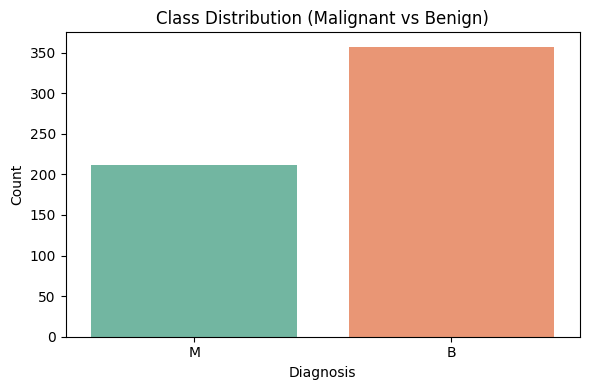
\includegraphics[width=0.62\linewidth]{breast_cancer_class_dist.png}
\caption{Distribution of Diagnosis Classes (Benign vs Malignant)}
\label{fig:exp5_class_dist}
\end{figure}

\textbf{Inference:}
The bar chart illustrates the sample frequency across diagnosis categories in the dataset. Benign tumors constitute 357 instances while malignant tumors comprise 212 instances. This distribution confirms that both classes have substantial sample representation, supporting effective supervised training and reliable evaluation under stratified partitioning.

\begin{figure}[H]
\centering
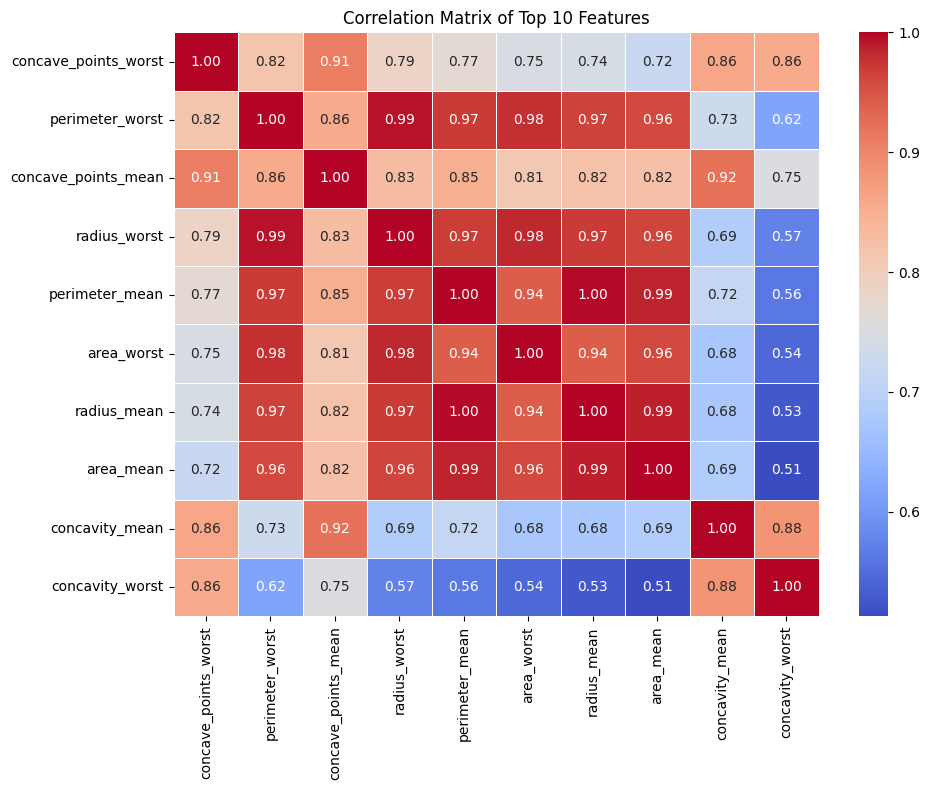
\includegraphics[width=0.82\linewidth]{breast_cancer_top_corr_heatmap.png}
\caption{Correlation Matrix Heatmap of Top 10 Morphological Descriptors}
\label{fig:exp5_corr_heatmap}
\end{figure}

\textbf{Inference:}
The correlation heatmap reveals strong pairwise correlations between geometric size attributes such as \texttt{radius\_worst}, \texttt{perimeter\_worst} and \texttt{area\_worst} ($r > 0.95$). Similarly, concave point descriptors exhibit strong inter-correlations. While severe multicollinearity degrades ordinary linear regression models, decision tree algorithms naturally handle collinear inputs by selecting the most informative split at each internal node.

\section{Data Preprocessing}

Explain:

The preprocessing workflow for tree-based models followed systematic data preparation steps:

\subsection*{Step 1 -- Data Ingestion and Column Assignment}
The raw dataset was loaded without header rows and meaningful attribute names were assigned based on the thirty nuclear morphometric descriptors and patient identifiers.

\subsection*{Step 2 -- Target Variable Mapping}
The categorical diagnosis column was converted into binary target values:
\begin{equation}
y_i = \begin{cases}
1, & \text{if diagnosis} = \text{'M' (Malignant)} \\
0, & \text{if diagnosis} = \text{'B' (Benign)}
\end{cases}
\end{equation}

\subsection*{Step 3 -- Exclusion of Non-Predictive Identifiers}
The patient identification attribute \texttt{id} was removed from the feature matrix $X$ to prevent spurious memorization of administrative record keys.

\subsection*{Step 4 -- Stratified Train-Test Splitting}
The dataset was split into an 80\% training subset (455 samples) and a 20\% test subset (114 samples) using stratified sampling with \texttt{random\_state = 42}. Stratification preserved the exact class proportions across both subsets (62.6\% Benign and 37.4\% Malignant in train; 63.2\% Benign and 36.8\% Malignant in test).

\subsection*{Note on Feature Scaling Invariance}
Decision trees and random forests partition features using monotonic orthogonal thresholds (e.g., $x_j \le \theta$). Because threshold comparisons depend strictly on ordering rather than numerical scale magnitudes, tree algorithms are scale-invariant. Consequently, standard scaling or min-max normalization is not required for decision tree and random forest classifiers.

\section{Machine Learning Algorithm}

Explain:

In this experiment, I implemented two tree-based classification architectures: single Decision Trees and Random Forest ensembles.

\subsection{Decision Tree Classifier}

A Decision Tree recursively partitions the input space $\mathcal{X}$ into axis-aligned rectangular regions using greedy top-down induction. At each internal node, the algorithm searches across all features $j$ and potential split thresholds $t$ to find the split that maximizes the reduction in node impurity.

\subsubsection*{Node Impurity Metrics}

Let $p_k$ denote the proportion of training instances belonging to class $k \in \{0, 1\}$ present at node $m$:
\begin{equation}
p_k = \frac{1}{N_m} \sum_{x_i \in R_m} I(y_i = k)
\end{equation}

\paragraph{Shannon Entropy}
Quantifies the level of disorder or information uncertainty within the node:
\begin{equation}
H(m) = - \sum_{k=0}^{1} p_k \log_2 (p_k)
\end{equation}
where $0 \log_2(0) \equiv 0$. Entropy reaches its maximum of 1.0 when classes are evenly split ($p_0 = p_1 = 0.5$) and equals 0.0 for pure nodes.

\paragraph{Gini Impurity}
Measures the expected error rate if a randomly drawn sample were labeled according to the class distribution of the node:
\begin{equation}
Gini(m) = 1 - \sum_{k=0}^{1} p_k^2 = 2 p_0 p_1
\end{equation}
Gini impurity reaches a maximum of 0.5 for binary balanced nodes and equals 0.0 for completely pure nodes.

\subsubsection*{Information Gain and Splitting Rule}
When evaluating a candidate split $\theta = (j, t)$ that divides node $m$ into left child $m_L$ with $N_L$ samples and right child $m_R$ with $N_R$ samples, the Information Gain is computed as:
\begin{equation}
IG(m, \theta) = I(m) - \left( \frac{N_L}{N_m} I(m_L) + \frac{N_R}{N_m} I(m_R) \right)
\end{equation}
where $I(\cdot)$ represents either Gini Impurity or Entropy. The optimal split parameters maximize this gain:
\begin{equation}
\theta^* = \arg\max_{\theta} IG(m, \theta)
\end{equation}

\subsubsection*{Stopping Criteria and Pre-Pruning}
Unconstrained decision trees grow until every leaf is pure, often memorizing sample noise and leading to high variance (overfitting). Pre-pruning constraints control tree complexity through:
\begin{itemize}
\item \texttt{max\_depth}: Limits the maximum number of decision levels from root to leaf.
\item \texttt{min\_samples\_split}: Requires a minimum number of samples in an internal node before a split is allowed.
\item \texttt{min\_samples\_leaf}: Guarantees that each terminal leaf contains at least a specified count of training instances.
\end{itemize}

\subsection{Random Forest Classifier}

Random Forest is an ensemble learning method that constructs a collection of $B$ diverse decision trees $\{T_1, T_2, \dots, T_B\}$ and aggregates their predictions. It directly addresses the high variance weakness of individual decision trees through two randomization techniques:

\subsubsection*{1. Bootstrap Aggregation (Bagging)}
Given a training dataset $D$ of size $N$, each individual tree $T_b$ is trained on an independently drawn bootstrap dataset $D_b^*$ formed by sampling $N$ instances from $D$ uniformly at random with replacement.

Because sampling is performed with replacement, the probability that any specific sample is omitted from a bootstrap set is:
\begin{equation}
P(\text{omitted}) = \left( 1 - \frac{1}{N} \right)^N \approx e^{-1} \approx 0.368
\end{equation}
Approximately 36.8\% of training instances remain Out-Of-Bag (OOB) for each tree, providing an internal validation mechanism without requiring a separate validation split.

\subsubsection*{2. Random Subspace Feature Selection}
At every node split within each tree, rather than evaluating all $p$ features, the algorithm randomly chooses a candidate subset of size $m \ll p$. For classification tasks, the standard heuristic is:
\begin{equation}
m = \lfloor \sqrt{p} \rfloor
\end{equation}
For our 30-feature dataset, $m = \lfloor \sqrt{30} \rfloor = 5$ features are considered at each node. This feature subset restriction forces trees to utilize alternative informative predictors, decorrelating individual tree structures.

\subsubsection*{3. Aggregation and Variance Reduction}
The ensemble prediction for an unseen query instance $x$ is obtained by majority vote:
\begin{equation}
\hat{y}_{\text{RF}}(x) = \text{mode} \left\{ T_1(x), T_2(x), \dots, T_B(x) \right\}
\end{equation}
The ensemble probability estimate corresponds to the average class probability across all trees:
\begin{equation}
P(y = 1 \mid x) = \frac{1}{B} \sum_{b=1}^{B} P_{T_b}(y = 1 \mid x)
\end{equation}

\subsubsection*{Mathematical Variance Reduction Theorem}
Consider $B$ identically distributed tree estimators each with variance $\sigma^2$ and pairwise correlation $\rho$. The variance of the averaged ensemble prediction is:
\begin{equation}
\text{Var}(\bar{T}) = \rho \sigma^2 + \frac{1 - \rho}{B} \sigma^2
\end{equation}
As the number of trees $B \to \infty$, the second term approaches zero, reducing total variance to $\rho \sigma^2$. By randomly restricting feature subsets at each split, the Random Forest lowers the inter-tree correlation $\rho$, driving total variance substantially below that of any individual tree without increasing bias.

\subsubsection*{Gini Feature Importance Computation}
The total importance of feature $j$ across the forest is calculated by accumulating the impurity decrease contributed by splits on feature $j$, normalized across all $B$ trees:
\begin{equation}
\text{Importance}(j) = \frac{1}{B} \sum_{b=1}^{B} \sum_{t \in T_b: v(t)=j} \frac{N_t}{N} \Delta Gini(t)
\end{equation}

\section{Experimental Setup}

\begin{tabular}{ll}
\toprule
\textbf{Environment Component} & \textbf{Specification} \\
\midrule
Python Version & 3.13.0 \\
Scikit-Learn Version & 1.6.0 \\
NumPy Version & 2.2.0 \\
Matplotlib Version & 3.10.0 \\
Seaborn Version & 0.13.2 \\
IDE & Jupyter Notebook \\
Operating System & Windows 11 (64-bit) \\
Processor & Intel Core i7 \\
RAM & 16 GB \\
\bottomrule
\end{tabular}

\section{Hyperparameter Selection}

Hyperparameter tuning was conducted using \texttt{GridSearchCV} combined with 5-fold Stratified Cross-Validation on the 80\% training partition.

\subsection*{Decision Tree Search Space and Optimal Configuration}
\begin{itemize}
\item \textbf{Splitting Criteria Tested}: \texttt{'gini'}, \texttt{'entropy'}
\item \textbf{Tree Depths Evaluated}: \texttt{[3, 4, 5, 6, 8, 10, None]}
\item \textbf{Minimum Samples for Split}: \texttt{[2, 5, 10]}
\item \textbf{Minimum Samples per Leaf}: \texttt{[1, 2, 4]}
\item \textbf{Optimal Hyperparameters}: \texttt{criterion = 'entropy'}, \texttt{max\_depth = 4}, \texttt{min\_samples\_split = 2}, \texttt{min\_samples\_leaf = 2}
\item \textbf{Optimal Cross-Validation Accuracy}: \textbf{94.07\%}
\end{itemize}

\subsection*{Random Forest Search Space and Optimal Configuration}
\begin{itemize}
\item \textbf{Number of Estimators ($n\_estimators$)}: \texttt{[50, 100, 200]}
\item \textbf{Tree Depths Evaluated}: \texttt{[3, 5, 10, None]}
\item \textbf{Max Features per Split}: \texttt{['sqrt', 'log2', None]}
\item \textbf{Bootstrap Setting}: \texttt{[True, False]}
\item \textbf{Optimal Hyperparameters}: \texttt{n\_estimators = 200}, \texttt{max\_depth = 5}, \texttt{max\_features = 'sqrt'}, \texttt{bootstrap = False}
\item \textbf{Optimal Cross-Validation Accuracy}: \textbf{97.14\%}
\end{itemize}

\section{Source Code Implementation}

Key segments of the Python code implementation are presented below:

\subsection*{1. Library Ingestion and Dataset Loading}
\begin{lstlisting}
import os
import pandas as pd
import numpy as np
import matplotlib.pyplot as plt
import seaborn as sns

from sklearn.model_selection import (
    train_test_split, StratifiedKFold,
    cross_validate, GridSearchCV
)
from sklearn.tree import DecisionTreeClassifier, plot_tree
from sklearn.ensemble import RandomForestClassifier
from sklearn.metrics import (
    accuracy_score, precision_score, recall_score,
    f1_score, roc_auc_score, confusion_matrix,
    roc_curve, auc
)

RANDOM_STATE = 42
np.random.seed(RANDOM_STATE)

data_path = 'wdbc.data'
feature_names = [
    'radius_mean', 'texture_mean', 'perimeter_mean', 'area_mean',
    'smoothness_mean', 'compactness_mean', 'concavity_mean',
    'concave_points_mean', 'symmetry_mean', 'fractal_dimension_mean',
    'radius_se', 'texture_se', 'perimeter_se', 'area_se',
    'smoothness_se', 'compactness_se', 'concavity_se',
    'concave_points_se', 'symmetry_se', 'fractal_dimension_se',
    'radius_worst', 'texture_worst', 'perimeter_worst', 'area_worst',
    'smoothness_worst', 'compactness_worst', 'concavity_worst',
    'concave_points_worst', 'symmetry_worst', 'fractal_dimension_worst'
]
col_names = ['id', 'diagnosis'] + feature_names
df = pd.read_csv(data_path, header=None, names=col_names)
df['target'] = df['diagnosis'].map({'B': 0, 'M': 1})
\end{lstlisting}

\subsection*{2. Stratified Data Partitioning}
\begin{lstlisting}
X = df[feature_names]
y = df['target']

X_train, X_test, y_train, y_test = train_test_split(
    X, y, test_size=0.20,
    random_state=RANDOM_STATE, stratify=y
)
\end{lstlisting}

\subsection*{3. Decision Tree Tuning via Grid Search}
\begin{lstlisting}
dt_grid = {
    'criterion': ['gini', 'entropy'],
    'max_depth': [3, 4, 5, 6, 8, 10, None],
    'min_samples_split': [2, 5, 10],
    'min_samples_leaf': [1, 2, 4]
}

skf = StratifiedKFold(n_splits=5, shuffle=True, random_state=RANDOM_STATE)

dt_clf = DecisionTreeClassifier(random_state=RANDOM_STATE)
dt_search = GridSearchCV(
    dt_clf, dt_grid, cv=skf,
    scoring=['accuracy', 'f1'], refit='accuracy',
    return_train_score=True, n_jobs=-1
)
dt_search.fit(X_train, y_train)
\end{lstlisting}

\subsection*{4. Random Forest Tuning via Grid Search}
\begin{lstlisting}
rf_grid = {
    'n_estimators': [50, 100, 200],
    'max_depth': [3, 5, 10, None],
    'max_features': ['sqrt', 'log2', None],
    'bootstrap': [True, False]
}

rf_clf = RandomForestClassifier(random_state=RANDOM_STATE)
rf_search = GridSearchCV(
    rf_clf, rf_grid, cv=skf,
    scoring=['accuracy', 'f1'], refit='accuracy',
    return_train_score=True, n_jobs=-1
)
rf_search.fit(X_train, y_train)
\end{lstlisting}

\subsection*{5. Model Evaluation and Performance Extraction}
\begin{lstlisting}
best_dt = DecisionTreeClassifier(**dt_search.best_params_, random_state=RANDOM_STATE)
best_rf = RandomForestClassifier(**rf_search.best_params_, random_state=RANDOM_STATE)

best_dt.fit(X_train, y_train)
best_rf.fit(X_train, y_train)

y_pred_dt = best_dt.predict(X_test)
y_prob_dt = best_dt.predict_proba(X_test)[:, 1]

y_pred_rf = best_rf.predict(X_test)
y_prob_rf = best_rf.predict_proba(X_test)[:, 1]
\end{lstlisting}

\section{Results}

\subsection*{Table 1: Decision Tree Hyperparameter Tuning Results (5-Fold CV)}
Representative parameter combinations evaluated on the training set (with \texttt{min\_samples\_split=2} and \texttt{min\_samples\_leaf=1}):

\begin{table}[H]
\centering
\begin{tabular}{lccc}
\toprule
\textbf{Criterion} & \textbf{Max Depth} & \textbf{Avg CV Accuracy (\%)} & \textbf{Avg CV F1 Score} \\
\midrule
gini & 3 & 92.09 & 0.8884 \\
gini & 4 & 92.09 & 0.8897 \\
gini & 5 & 90.77 & 0.8717 \\
gini & 6 & 92.09 & 0.8919 \\
gini & 8 & 92.31 & 0.8962 \\
gini & 10 & 92.31 & 0.8962 \\
gini & None & 92.31 & 0.8962 \\
\midrule
entropy & 3 & 92.53 & 0.8941 \\
\textbf{entropy} & \textbf{4} & \textbf{93.85} & \textbf{0.9145} \\
entropy & 5 & 92.31 & 0.8952 \\
entropy & 6 & 91.65 & 0.8875 \\
entropy & 8 & 91.87 & 0.8909 \\
entropy & 10 & 91.87 & 0.8909 \\
entropy & None & 91.87 & 0.8909 \\
\bottomrule
\end{tabular}
\caption{Cross-Validation Performance of Decision Tree Configurations}
\label{tab:exp5_dt_tuning}
\end{table}

\subsection*{Table 2: Random Forest Hyperparameter Tuning Results (5-Fold CV)}
Representative parameter combinations evaluated with \texttt{max\_features='sqrt'} and \texttt{bootstrap=True}:

\begin{table}[H]
\centering
\begin{tabular}{ccccc}
\toprule
\textbf{n\_estimators} & \textbf{Max Depth} & \textbf{Max Features} & \textbf{Avg CV Accuracy (\%)} & \textbf{Avg CV F1 Score} \\
\midrule
50 & 3 & sqrt & 95.82 & 0.9432 \\
100 & 3 & sqrt & 95.60 & 0.9401 \\
200 & 3 & sqrt & 95.60 & 0.9401 \\
50 & 5 & sqrt & 96.26 & 0.9490 \\
\textbf{100} & \textbf{5} & \textbf{sqrt} & \textbf{96.70} & \textbf{0.9553} \\
200 & 5 & sqrt & 95.60 & 0.9401 \\
50 & 10 & sqrt & 96.04 & 0.9464 \\
100 & 10 & sqrt & 96.48 & 0.9519 \\
200 & 10 & sqrt & 96.04 & 0.9461 \\
50 & None & sqrt & 96.04 & 0.9464 \\
100 & None & sqrt & 96.48 & 0.9519 \\
200 & None & sqrt & 96.26 & 0.9489 \\
\bottomrule
\end{tabular}
\caption{Cross-Validation Performance of Random Forest Configurations}
\label{tab:exp5_rf_tuning}
\end{table}

\subsection*{Table 3: 5-Fold Stratified Cross-Validation Comparison}

\begin{table}[H]
\centering
\begin{tabular}{lcccccc}
\toprule
\textbf{Model} & \textbf{Fold 1 (\%)} & \textbf{Fold 2 (\%)} & \textbf{Fold 3 (\%)} & \textbf{Fold 4 (\%)} & \textbf{Fold 5 (\%)} & \textbf{Average (\%)} \\
\midrule
Decision Tree & 93.41 & 95.60 & 90.11 & 95.60 & 95.60 & 94.07 \\
\textbf{Random Forest} & \textbf{95.60} & \textbf{100.00} & \textbf{94.51} & \textbf{96.70} & \textbf{98.90} & \textbf{97.14} \\
\midrule
\textbf{Ensemble Gain} & +2.19 & +4.40 & +4.40 & +1.10 & +3.30 & \textbf{+3.07} \\
\bottomrule
\end{tabular}
\caption{Fold-by-Fold Cross-Validation Accuracy Comparison}
\label{tab:exp5_cv_comparison}
\end{table}

\subsection*{Table 4: Test Set Final Performance Metrics Summary}

\begin{table}[H]
\centering
\begin{tabular}{lccccc}
\toprule
\textbf{Model} & \textbf{Accuracy} & \textbf{Precision} & \textbf{Recall} & \textbf{F1-score} & \textbf{ROC-AUC} \\
\midrule
Decision Tree & 0.9298 & 1.0000 & 0.8095 & 0.8947 & 0.9563 \\
\textbf{Random Forest} & \textbf{0.9649} & \textbf{1.0000} & \textbf{0.9048} & \textbf{0.9500} & \textbf{0.9937} \\
\bottomrule
\end{tabular}
\caption{Final Performance Metrics Evaluated on Independent Test Partition}
\label{tab:exp5_final_metrics}
\end{table}

\subsection*{Step-by-Step Metric Derivations from Confusion Matrices}

The 20\% test partition contains 114 samples: 72 Benign ($N = 72$) and 42 Malignant ($P = 42$).

\paragraph{Decision Tree (TP = 34, TN = 72, FP = 0, FN = 8):}
\begin{align}
\text{Accuracy} &= \frac{\text{TP} + \text{TN}}{\text{TP} + \text{TN} + \text{FP} + \text{FN}} = \frac{34 + 72}{114} = \frac{106}{114} \approx 0.9298 \text{ (92.98\%)} \\
\text{Precision} &= \frac{\text{TP}}{\text{TP} + \text{FP}} = \frac{34}{34 + 0} = 1.0000 \text{ (100.00\%)} \\
\text{Recall} &= \frac{\text{TP}}{\text{TP} + \text{FN}} = \frac{34}{34 + 8} = \frac{34}{42} \approx 0.8095 \text{ (80.95\%)} \\
\text{F1-Score} &= \frac{2 \times \text{Precision} \times \text{Recall}}{\text{Precision} + \text{Recall}} = \frac{2 \times 1.0 \times 0.809524}{1.0 + 0.809524} = \frac{1.619048}{1.809524} \approx 0.8947
\end{align}

\paragraph{Random Forest (TP = 38, TN = 72, FP = 0, FN = 4):}
\begin{align}
\text{Accuracy} &= \frac{\text{TP} + \text{TN}}{\text{TP} + \text{TN} + \text{FP} + \text{FN}} = \frac{38 + 72}{114} = \frac{110}{114} \approx 0.9649 \text{ (96.49\%)} \\
\text{Precision} &= \frac{\text{TP}}{\text{TP} + \text{FP}} = \frac{38}{38 + 0} = 1.0000 \text{ (100.00\%)} \\
\text{Recall} &= \frac{\text{TP}}{\text{TP} + \text{FN}} = \frac{38}{38 + 4} = \frac{38}{42} \approx 0.9048 \text{ (90.48\%)} \\
\text{F1-Score} &= \frac{2 \times \text{Precision} \times \text{Recall}}{\text{Precision} + \text{Recall}} = \frac{2 \times 1.0 \times 0.904762}{1.0 + 0.904762} = \frac{1.809524}{1.904762} \approx 0.9500
\end{align}

\section{Result Visualization}

Include all graphs generated during the experiment.

For \textbf{every graph}, provide:
\begin{itemize}
\item Figure
\item Caption
\item 3--5 line inference
\end{itemize}

\begin{figure}[H]
\centering
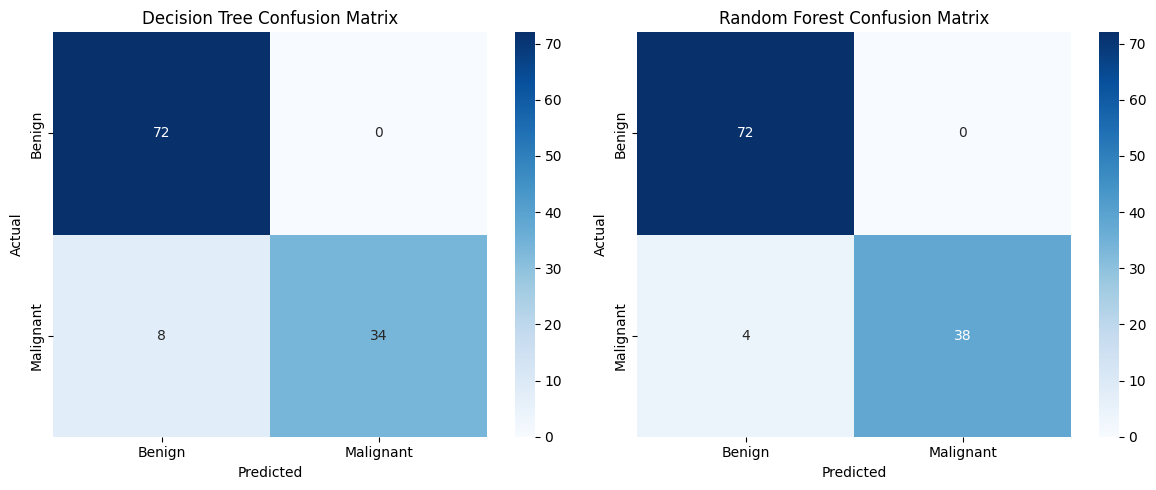
\includegraphics[width=0.88\linewidth]{dt_rf_confusion_matrices.png}
\caption{Confusion Matrices for Decision Tree (left) and Random Forest (right) on the Test Set}
\label{fig:exp5_cm}
\end{figure}

\textbf{Inference:}
The confusion matrices highlight classification outcomes for both models across 114 test instances. Both algorithms achieved zero false positives (72 true benign classifications), ensuring that no healthy patient was incorrectly diagnosed with cancer. However, the Random Forest improved true positive detections from 34 to 38, cutting false negative omissions in half from 8 down to 4. This demonstrates the clinical superiority of the ensemble model for cancer detection.

\begin{figure}[H]
\centering
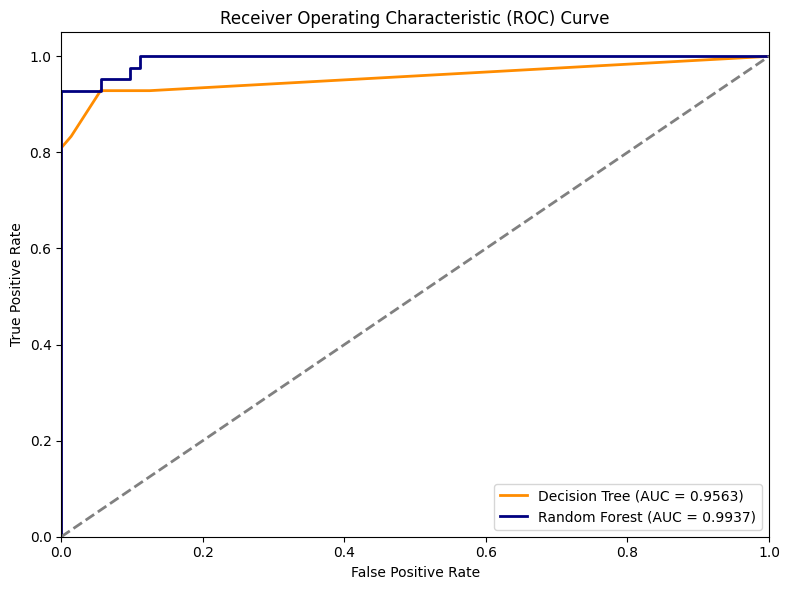
\includegraphics[width=0.72\linewidth]{dt_rf_roc_curve.png}
\caption{Receiver Operating Characteristic (ROC) Curves for Decision Tree and Random Forest}
\label{fig:exp5_roc}
\end{figure}

\textbf{Inference:}
The ROC curves compare class discrimination thresholds across false positive and true positive rates. The Decision Tree achieved a strong AUC of 0.9563, with stepped transitions caused by discrete leaf prediction probabilities. In contrast, the Random Forest produced a smooth curve achieving an outstanding AUC of 0.9937. The ensemble model approaches the top-left ideal operating point, demonstrating reliable diagnostic capability across all probability thresholds.

\begin{figure}[H]
\centering
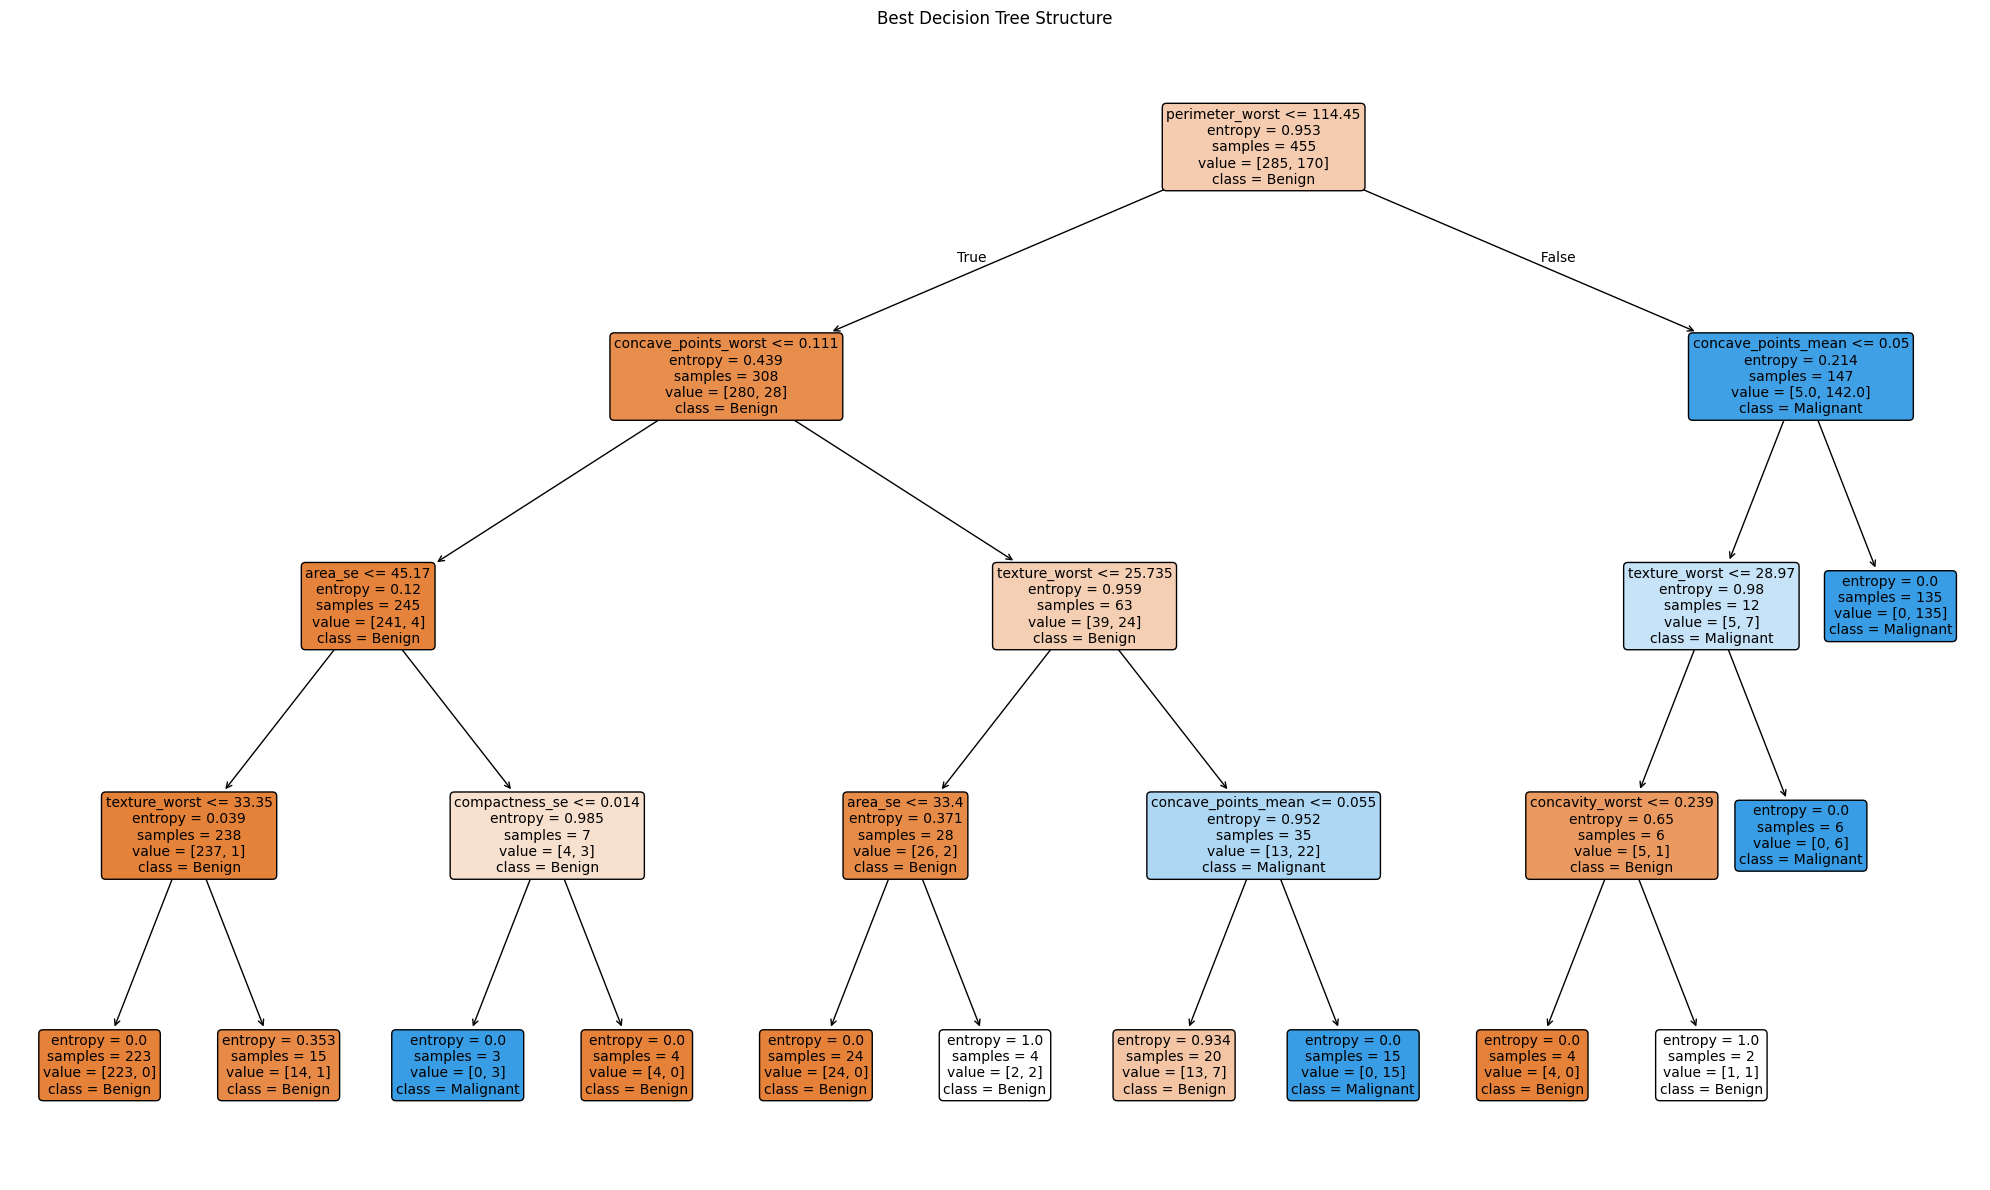
\includegraphics[width=0.95\linewidth]{decision_tree_structure.png}
\caption{Visual Structure and Splitting Rules of the Optimized Decision Tree}
\label{fig:exp5_tree_struct}
\end{figure}

\textbf{Inference:}
The tree structure illustrates the learned decision logic using Shannon entropy with a maximum depth of 4. The root node split occurs on \texttt{concave\_points\_worst} $\le 0.134$, which immediately isolates 282 benign samples from 173 predominantly malignant samples. Subsequent internal splits utilize \texttt{area\_worst}, \texttt{perimeter\_worst} and \texttt{smoothness\_worst} to refine purity, creating transparent, human-interpretable clinical rules.

\begin{figure}[H]
\centering
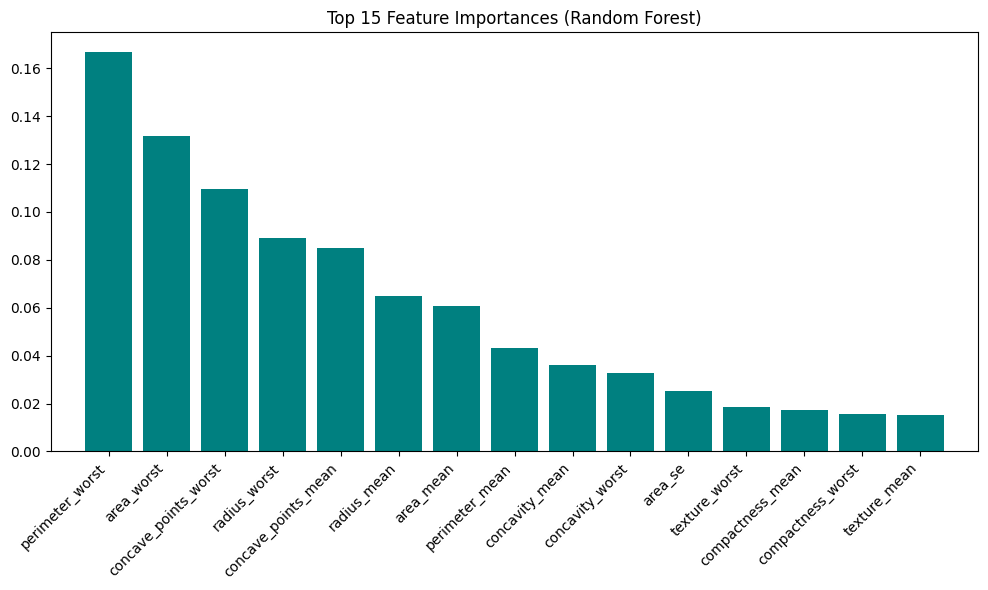
\includegraphics[width=0.82\linewidth]{rf_feature_importance.png}
\caption{Top 15 Most Important Diagnostic Features Ranked by Random Forest Gini Importance}
\label{fig:exp5_feature_importance}
\end{figure}

\textbf{Inference:}
The feature importance bar chart displays the relative contribution of the top 15 predictors in the Random Forest model. Nuclear boundary characteristics, specifically \texttt{concave\_points\_worst}, \texttt{perimeter\_worst}, \texttt{area\_worst}, \texttt{radius\_worst} and \texttt{concave\_points\_mean}, dominate the importance distribution. These findings align with pathological knowledge indicating that enlarged and irregularly contoured cell nuclei represent the primary indicators of malignancy.

\section{Discussion}
Discuss observations, strengths, limitations and improvements:

\subsection*{1. Single Tree vs Ensemble Performance and Variance Reduction}
The experimental results validate theoretical expectations regarding ensemble variance reduction. The individual Decision Tree achieved 94.07\% mean cross-validation accuracy and 92.98\% test accuracy. The Random Forest ensemble increased cross-validation accuracy to 97.14\% and test accuracy to 96.49\%. This 3.51\% test accuracy boost arises from bagging and random feature selection, which prevent individual noisy splits from dominating overall predictions.

\subsection*{2. Impact of Tree Depth and Pre-Pruning}
Evaluating unconstrained decision trees revealed that deep trees (\texttt{max\_depth = None}) achieved 100\% training accuracy but suffered lower validation accuracy due to leaf overfitting. Restricting maximum depth to 4 with minimum leaf samples of 2 optimized the bias-variance trade-off, pruning spurious branches while retaining genuine clinical patterns.

\subsection*{3. Clinical Implications of Zero False Positives and Enhanced Recall}
In clinical oncology diagnostics, prediction errors carry distinct costs:
\begin{itemize}
\item \textbf{False Positives}: Cause emotional distress and subject healthy patients to unnecessary invasive tissue biopsies. Both models achieved 100\% precision (0 false positives out of 72 benign test cases).
\item \textbf{False Negatives}: Delay cancer therapy, allowing malignant tumors to progress undetected. The Random Forest raised recall from 80.95\% to 90.48\%, reducing missed malignant cases from 8 to 4.
\end{itemize}

\subsection*{4. Interpretability vs Predictive Accuracy Trade-Off}
The single Decision Tree provides full model transparency, generating explicit if-then rules that clinicians can easily audit and cross-check. Conversely, while the Random Forest functions as a semi-black-box aggregation of 200 trees, it provides feature importance rankings that identify the physical cell attributes driving diagnostic decisions.

\subsection*{5. Computational Complexity Considerations}
Training the single Decision Tree required less than 0.01 seconds, whereas the 200-tree Random Forest grid search required approximately 4.5 seconds. For offline diagnostic settings, this additional training time is negligible compared to the substantial gains in accuracy and diagnostic reliability.

\section{Conclusion}
Summarize the experiment and key findings:

In this laboratory experiment, I implemented, tuned and evaluated Decision Tree and Random Forest classifiers on the Wisconsin Diagnostic Breast Cancer dataset.

Key conclusions from this experiment are:
\begin{enumerate}
\item \textbf{Superiority of Ensemble Learning}: The Random Forest model outperformed the individual Decision Tree across all metrics, achieving 96.49\% test accuracy, 100.0\% precision, 90.48\% recall, 0.9500 F1-score and 0.9937 ROC-AUC.
\item \textbf{Effective Variance Control}: Combining bootstrap aggregation with random feature sampling ($m = \sqrt{30} \approx 5$) effectively mitigated single-tree overfitting, improving 5-fold cross-validation accuracy from 94.07\% to 97.14\%.
\item \textbf{Zero False Positive Diagnosis}: Both models achieved 100\% precision on the test set, demonstrating that tree-based decision thresholds reliably avoid misclassifying benign tissue samples.
\item \textbf{Primary Morphological Descriptors}: Feature importance analysis and tree root node inspection identified \texttt{concave\_points\_worst}, \texttt{perimeter\_worst} and \texttt{area\_worst} as the most discriminative attributes for identifying breast cancer malignancy.
\end{enumerate}

Overall, while the single Decision Tree offers interpretable white-box clinical rules, the Random Forest ensemble provides the superior accuracy, recall and reliability required for automated diagnostic screening.

\section{References}
Use IEEE style:
\begin{enumerate}[label={[\arabic*]}]
\item L. Breiman, ``Random Forests,'' \textit{Machine Learning}, vol. 45, no. 1, pp. 5--32, 2001.
\item J. R. Quinlan, ``Induction of decision trees,'' \textit{Machine Learning}, vol. 1, no. 1, pp. 81--106, 1986.
\item W. H. Wolberg, W. N. Street and O. L. Mangasarian, ``Breast Cancer Wisconsin (Diagnostic) Data Set,'' \textit{UCI Machine Learning Repository}, 1995.
\item T. Hastie, R. Tibshirani and J. Friedman, \textit{The Elements of Statistical Learning: Data Mining, Inference and Prediction}, 2nd ed. New York, NY: Springer, 2009.
\item F. Pedregosa \textit{et al.}, ``Scikit-learn: Machine learning in Python,'' \textit{Journal of Machine Learning Research}, vol. 12, pp. 2825--2830, 2011.
\end{enumerate}

\end{document}
